\section{Testiprojektista}

\subsection{Yksikkötestidemo}

\begin{figure}[htb]
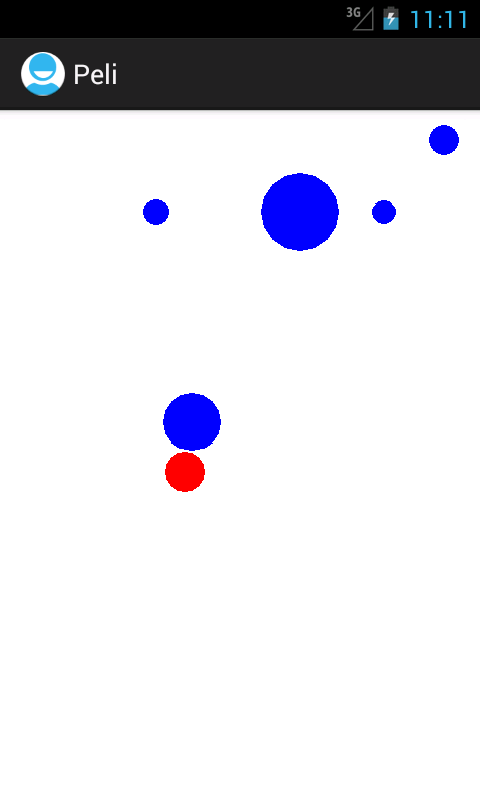
\includegraphics[width=60mm]{peli_screenshot.png}
\caption{Ruutukaappaus pelist} \label{peli_screenshot}
\end{figure}

Yksikkötestaustyökaluja testasin itse tehdyllä demoprojektilla. Kyseessä on yksinkertainen peli, jonka pelinäkymästä on ruutukaappaus kuvassa \ref{peli_screenshot}. Pelissä ohjataan kosketusnäytöllä painamalla punaista palloa ja pyritään väistämään ympäriinsä pomppivia sinisiä palloja. Kun peli päättyy, palataan takaisin päänäkymään, josta on ruutukaappaus kuvassa \ref{mainactivity}. Tästä näkymästä voi aloittaa uuden pelin ja lisäksi näkee, montako sekuntia edellinen peli kesti.

\begin{figure}[htb]
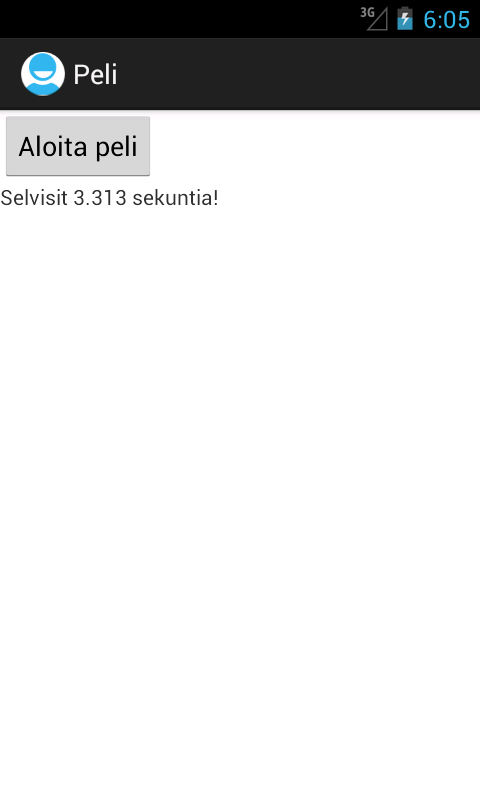
\includegraphics[width=60mm]{peli_mainactivity.png}
\caption{Ruutukaappaus pelist} \label{mainactivity}
\end{figure}

Peli koostuu kahdesta aktiviteetista, yksinkertaisemmasta MainActivity:sta sekä hieman monimutkaisemmasta GameActivity:sta, jonka yksikkötestaukseen keskityn. Itse peliä ohjaa GameView-luokka, joka on yhtä aikaa näkymä ja kontrolleri MVC-suunnittelumallin mukaisesti. Malleja ovat GameClock, joka kuvaa pelikelloa, sekä Circle, joka kuvaa yhtä ruudulla näkyvää ympyrää. GameActivity toteuttaa lisäksi OnGameEndListener-rajapinnan, jonka avulla GameView ilmoittaa pelin päättymisestä ja pistemäärästä. Pelin luokkakaavio on esitetty kuvassa \ref{game_classdiagram}.

\begin{figure}[htb]
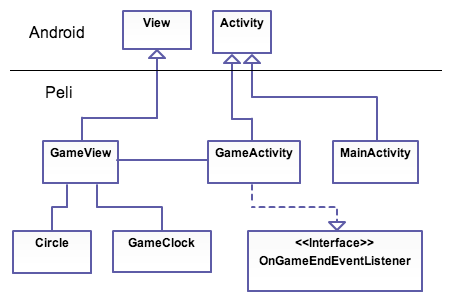
\includegraphics[width=110mm]{peli_luokkakaavio.png}
\caption{Pelin luokkakaavio} \label{game_classdiagram}
\end{figure}

\subsection{Tomdroidin toiminnallinen testaus}

\begin{figure}[htb]
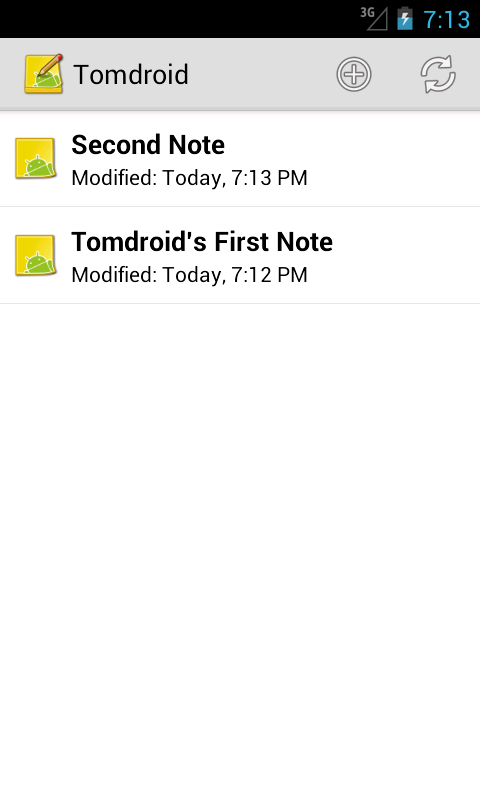
\includegraphics[width=60mm]{tomdroid_notelist.png}
\caption{Muistikirjalista Tomdroidissa} \label{tomdroid_notelist}
\end{figure}

Testityökalujen vertailussa käytän testattavana ohjelmana Tomdroidia. Tomdroid on GPL-lisenssillä julkaistu avoimen lähdekoodin sovellus, joka toimii muistikirjasovelluksena, joka synkronisoi sisältönsä automaattisesti. \cite{tomdroid} Tomdroid on valittu testattavaksi sovellukseksi, koska sen lähdekoodi on saatavilla, se on riittävän monimutkainen, jotta sille tehdyt testit kuvaisivat oikeassa android-kehityksessä kohdattavia testaushaasteita, se on vasta beta-vaiheessa, joten sovelluksesta pitäisi löytyä myös bugeja ja lisäksi sovelluksen oma testaus on lähes olematonta.

Tätä tutkimusta varten tein kopion tomdroidin lähdekoodista versiosta 0.7.2 ja kopioin sen githubiin. Sieltä löytyy myös kaikki tässä tutkimuksessa sovellukselle tehdyt testit. \cite{tomdroid_github}

Tomdroidissa olennaisimmat näkymät ovat muistikirjalista, josta on ruutukaappaus kuvassa \ref{tomdroid_notelist}, yksittäisen muistikirjan selaaminen (kuvassa \ref{tomdroid_noteview}) ja sen editointi (kuvassa \ref{tomdroid_editview}). 

Listanäkymässä näkyvät kaikki käyttäjän muistikirjat päivitysajan mukaan järjestettynä. Muistikirjan koskeminen avaa kyseisen muistikirjan selausnäkymän. Yläpalkin +-symboli luo uuden muistikirjan ja avaa sen editointinäkymään. Yläpalkin oikeassa reunassa on synkronointi-symboli, josta muistikirjojen tila päivitetään palvelimen kanssa.

Selausnäkymässä voi lukea yksittäistä muistikirjaa. Jos tekstiä on enemmän kuin ruudulle mahtuu kerrallaan, sitä voi selata raahaamalla. Kynä-ikoni yläpalkissa avaa muistikirjan editointinäkymään. Yläpalkin oikean reunan ikonista voi jakaa muistikirjan toisiin sovelluksiin. Lisäksi vasemman yläreunan ikonista pääsee takaisin listaan.

Editointinäkymässä yläpalkissa on kuvakkeet muutosten tallentamista ja perumista varten. Tallennettaessa ruudulla näkyy hetken aikaa leijuke, jossa kerrotaan muutosten tallennuksesta. Painettaessa peru-nappia ruudulle tulee dialogi, jossa pitää vahvistaa peruminen edelliseen tallennettuun versioon. Lisäksi vasemman yläreunan ikonista pääsee takaisin listaan.

\begin{figure}[htb]
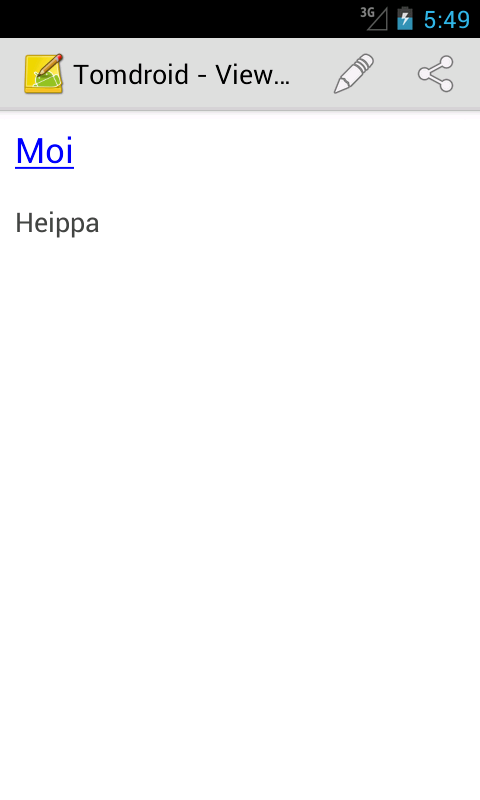
\includegraphics[width=60mm]{tomdroid_noteview.png}
\caption{Muistikirjan luku Tomdroidissa} \label{tomdroid_noteview}
\end{figure}

\begin{figure}[htb]
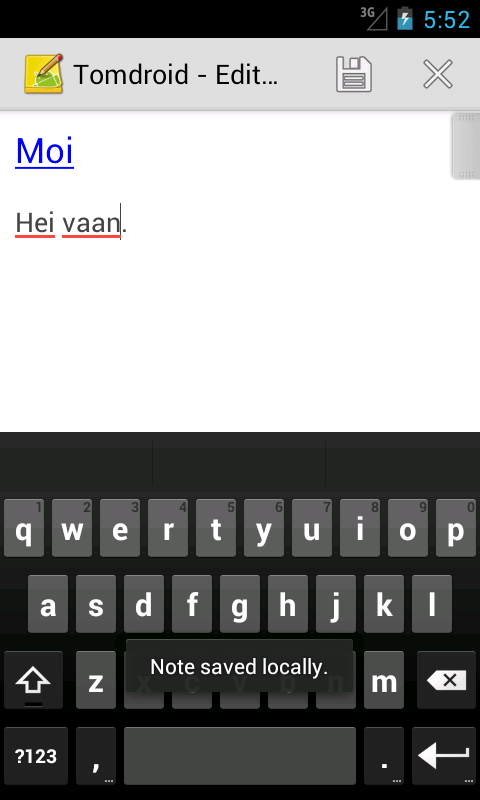
\includegraphics[width=60mm]{tomdroid_editview.png}
\caption{Muistikirjan editointi Tomdroidissa} \label{tomdroid_editview}
\end{figure}